\section{General Interface}

\subsection{Strokes}

A \emph{stroke} is a continuous set of points drawn on our system.
Since the system works both on Tablet PCs and on power walls,
a stroke can be drawn either with the tablet's pen or with
a regular laser pointer.

Drawing strokes is therefore the main way of users interaction with
the system. It has been built to support several users interacting
simultaneously in the screen.

With this approach, any component in the system can't make use
of global mode information due to the fact that one can't know
for sure if the $ stroke_{n+1} $ was drawn by the same user than $ stroke_{n} $.

Therefore, strokes must serve many purposes, and in cases where a sequence
of actions must be done in order, they're achieved under the same stroke.

Another decision taken early on in the implementation was that there shall not be
fixed areas in the screen for contents such as menus. The initial state of the
system is completely free of interface widgets. When starting the system the users
see only a 3D perspective of the virtual world.


\subsubsection{Stroke Actions}

Any stroke can be interpreted as being one of (see figure \ref{fig:lasso-tri}):

\begin{description}
		\item[an open stroke] --
				any stroke where the segments don't intercept each other;

		\item[a lasso] --
				a closed stroke;

		\item[a triangle stroke] --
				this is a special case of a lasso, i.e. closed, where the stroke resembles a triangle.
\end{description}


\begin{figure}[!ht]
		\centering
		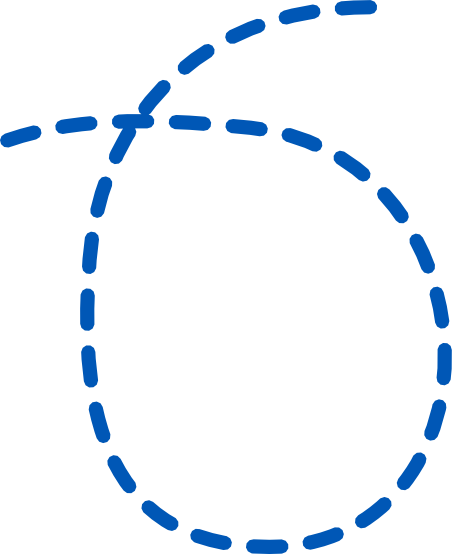
\includegraphics[width=3.5cm]{gfx/lasso.png}
		\qquad\qquad\qquad
		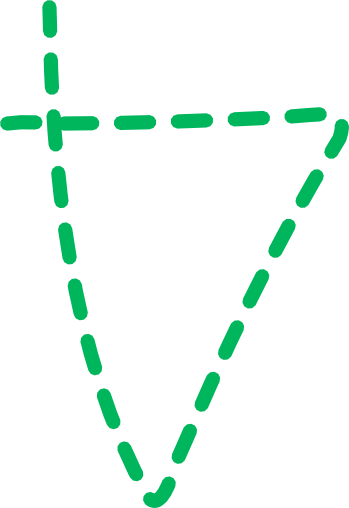
\includegraphics[width=3cm]{gfx/triangle.png}
		\caption{Lasso and triangle strokes}
		\label{fig:lasso-tri}
\end{figure}


\subsection{Gates}

As described earlier on in section \ref{sec:gate-concept} The Gate Concept,
a gate solves the problem of our input devices not being capable of detecting
click actions consistently.

\begin{figure}[!ht]
		\centering
		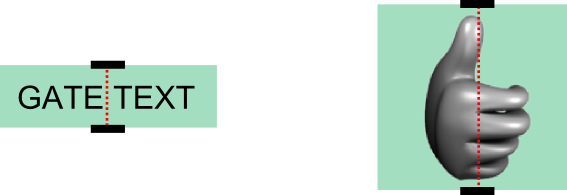
\includegraphics[width=5cm]{gfx/gate1e.png}
		\vspace{-0.5cm}
		\caption{Two gates: one featuring text and the other visual content}
		\label{fig:gate1}
\end{figure}

\begin{figure}[!ht]
		\vspace{-0.7cm}
		\centering
		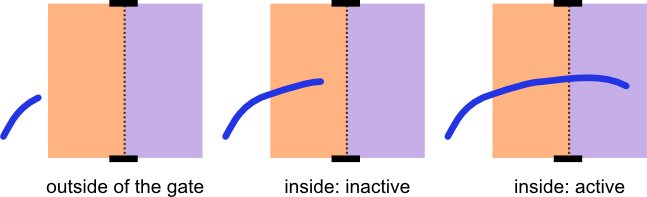
\includegraphics[width=10cm]{gfx/gate2e.png}
		\vspace{-0.5cm}
		\caption{Gate activation}
		\label{fig:gate2}
\end{figure}

\begin{figure}[!ht]
		\vspace{-0.7cm}
		\centering
		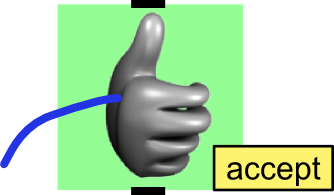
\includegraphics[width=3cm]{gfx/gate3e.png}
		\vspace{-0.5cm}
		\caption{Gate showing its tooltip}
		\label{fig:gate3}
\end{figure}


Gates can either have text our visual content (fig \ref{fig:gate1}).
It was decided that gates shouldn't feature both at the same time.

The activation takes place by entering both the left side and the right
side areas of the gate consecutively (or the other way around).
The dashed line in figure \ref{fig:gate2} is only imaginary.

In order for users to inspect the meaning a gate with visual content, a
tooltip appears when the stroke is inside the gate,
which will happen prior to activation, so users can give it up (figure \ref{fig:gate3}).



\subsection{Menus}
